\documentclass[border=3pt]{standalone}
% Preâmbulo compartilhado pelos diagramas TikZ da aula
\usepackage[T1]{fontenc}
\usepackage[utf8]{inputenc}
\usepackage{lmodern}
\usepackage{amsmath}
\usepackage{xcolor}
\usepackage{tikz}
\usetikzlibrary{arrows.meta,angles,quotes,decorations.pathmorphing,calc,
                positioning,shapes.geometric,backgrounds,fit}

% Paleta (mesma dos SVGs originais)
\definecolor{dblue}{HTML}{2A5B8C}
\definecolor{dorange}{HTML}{B3541E}
\definecolor{dgreen}{HTML}{4A7C59}
\definecolor{dred}{HTML}{9C4B4B}
\definecolor{dcream}{HTML}{F4F1EA}
\definecolor{dshade}{HTML}{DDD7C9}

% Estilos comuns (prefixo d... para não colidir com chaves internas do pgf)
\tikzset{
  >={Stealth[length=2mm]},
  dguide/.style={gray!55, dashed, line width=0.4pt},
  daxis/.style={gray!60, line width=0.7pt, ->},
  dbody/.style={fill=black!3, draw=black!80, line width=1pt},
  dacc/.style={draw=dblue, line width=1pt},
  dlbl/.style={black!55, font=\small},
  dsub/.style={black!45, font=\footnotesize},
  dstate/.style={circle, draw=black!80, fill=dcream, line width=1pt,
                 minimum size=17mm, font=\large, inner sep=1pt},
  dobs/.style={circle, draw=black!80, fill=dshade, line width=1pt,
               minimum size=14mm, font=\large, inner sep=1pt},
  dbox/.style={rounded corners=2pt, draw=black!80, fill=dcream, line width=1pt,
               align=center, inner sep=6pt},
  dtrans/.style={->, dblue, line width=1pt},
  dmeas/.style={->, dorange, line width=1pt},
}

\begin{document}
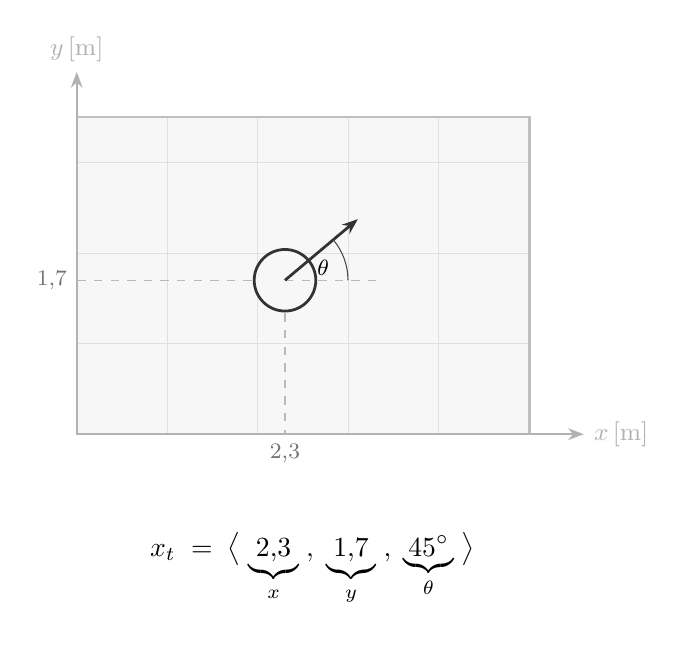
\begin{tikzpicture}[x=1.15cm,y=1.15cm]

  % piso / sala com grade
  \fill[black!3] (0,0) rectangle (5,3.5);
  \foreach \gx in {1,2,3,4} \draw[black!12, line width=0.4pt] (\gx,0) -- (\gx,3.5);
  \foreach \gy in {1,2,3}   \draw[black!12, line width=0.4pt] (0,\gy) -- (5,\gy);
  \draw[black!25, line width=0.8pt] (0,0) rectangle (5,3.5);

  % eixos
  \draw[daxis] (0,0) -- (5.6,0) node[right, font=\small] {$x$\,[m]};
  \draw[daxis] (0,0) -- (0,4.0) node[above, font=\small] {$y$\,[m]};

  % pose do robô
  \coordinate (R) at (2.3,1.7);
  \coordinate (H) at ($(R)+(40:1.05)$);
  \coordinate (Ref) at ($(R)+(1.0,0)$);

  \draw[dguide] (R) -- (2.3,0) node[below, black!55, font=\footnotesize] {$2{,}3$};
  \draw[dguide] (R) -- (0,1.7) node[left,  black!55, font=\footnotesize] {$1{,}7$};

  \draw[dbody] (R) circle (0.34);
  \draw[dguide] (R) -- (Ref);
  \draw[->, black!80, line width=1pt] (R) -- (H);
  \pic[draw=black!70, angle radius=8mm, "$\theta$" {font=\footnotesize, xshift=1pt}]
      {angle = Ref--R--H};

  % vetor de estado com componentes rotulados
  \node[anchor=north, font=\normalsize, inner sep=6pt] at (2.6,-0.9)
    {$x_t \;=\; \bigl\langle\;
        \underbrace{2{,}3}_{x}\;,\;
        \underbrace{1{,}7}_{y}\;,\;
        \underbrace{45^\circ}_{\theta}
      \;\bigr\rangle$};

\end{tikzpicture}
\end{document}
